\documentclass[a4paper]{report}
\usepackage{geometry}
\usepackage{graphics}
\usepackage{ifpdf}
\usepackage{makeidx}
\usepackage{fancyhdr}
\usepackage{fancyvrb}
\usepackage{amsmath, amsthm, amssymb}

\ifpdf
\pdfinfo{
  /Title    (Clus: User's Manual)
  /Author   (Jan Struyf, Bernard Zenko, Hendrik Blockeel, Saso Dzeroski)
}
\usepackage[pdftex,colorlinks=true,pdfstartview=FitV,linkcolor=black,citecolor=black,urlcolor=black]{hyperref}
\else
\usepackage{url}
\newcommand{\phantomsection}[1]{}
\fi

% geometry makes sure page size is correct in .pdf files
\geometry{a4paper,
          centering,
          textwidth = 16.5cm,
          textheight = 24.5cm
}

\renewcommand{\topfraction}{1.0}
\setcounter{topnumber}{4}
\setcounter{totalnumber}{4}
\renewcommand{\textfraction}{0.07}

\newcommand{\clus}{\textsc{Clus}}

\begin{document}

\title{Clus: User's Manual}

\author{Jan Struyf, Bernard \v{Z}enko, Hendrik Blockeel, Sa\v{s}o D\v{z}eroski}

\maketitle



\tableofcontents



\chapter{Introduction}

This text is a user's manual for the open source machine learning system \clus{}. \clus{} is a decision tree and rule learning system that works in the {\em predictive clustering} framework \cite{Blockeel1998icml}.

While most decision tree learners induce classification or regression trees, \clus{} generalizes this approach by learning trees that are interpreted as cluster hierarchies. We call such trees predictive clustering trees or PCTs. Depending on the learning task at hand, different goal criteria are to be optimized while creating the clusters, and different heuristics will be suitable to achieve this.

Classification and regression trees are special cases of PCTs, and by choosing the right parameter settings \clus{} can closely mimic the behavior of tree learners such as CART \cite{Breiman84:other} or C4.5 \cite{Quinlan93:other}.  However, its applicability goes well beyond classical classification or regression tasks: \clus{} has been successfully applied to many different tasks including multi-task learning (multi-target classification and regression), structured output learning, multi-label classification, hierarchical classification, and time series prediction. Next to these supervised learning tasks, PCTs are also applicable to semi-supervised learning, subgroup discovery, and clustering.

In a similar way, predictive clustering rules (PCRs) generalize classification rule sets \cite{Clark91:proc} and also apply to the aforementioned learning tasks.

A full description of how \clus{} works is beyond the scope of this text. In this User's Manual, we focus on how to use \clus{}: how to prepare its inputs, how to interpret the output, and how to change its behavior with the available parameters.

For background information on the rationale behind the \clus{} system and its algorithms we refer to the following papers:

\begin{itemize}

\item H. Blockeel, L. De Raedt, and J. Ramon, Top-down induction of clustering trees, Proceedings of the 15th International Conference on Machine Learning (Shavlik, J., ed.), pp. 55-63, 1998.

\item B.~{\v{Z}}enko and S.~D{\v{z}}eroski. Learning classification rules for multiple target attributes. In Advances in Knowledge Discovery and Data Mining, pp. 454-465, 2008.

\item H. Blockeel, S. D\v zeroski, and J. Grbovic, Simultaneous prediction of multiple chemical parameters of river water quality with TILDE, Proceedings of the Third European Conference on Principles of Data Mining and Knowledge Discovery (Zytkow, J.M. and Rauch, J., eds.), vol 1704, LNAI, pp. 32-40, 1999.

\item  C. Vens, J. Struyf, L. Schietgat, S. D\v zeroski and H. Blockeel, Decision trees for hierarchical multi-label classification. Machine Learning 73(2):185-214, 2008.
\end{itemize}

A longer list of publications describing applications of \clus{} is available on the \clus{} web site
(\url{www.cs.kuleuven.be/~dtai/clus/publications.html}).

\chapter{Tutorial}

\section{Installing and Running Clus}
\label{sec:run}

\begin{sloppypar}
\clus{} is written in the Java programming language, which is available from {\tt http://java.sun.com}. You will need Java version 1.5.x or above. To run \clus{}, it suffices to install the Java Runtime Environment (JRE). If you want to make changes to \clus{} and compile its source code, then you will need to install the Java Development Kit (JDK) instead of the JRE.
\end{sloppypar}

After downloading \clus{}, unpack it into a directory of your choice. \clus{} is a command line application and should be started from the command prompt (Windows) or a terminal window (Unix). To start \clus{}, enter the command:
\begin{flushleft}
\verb^java -jar $CLUS_DIR/Clus.jar^ {\em filename}\verb^.s^
\end{flushleft}

\noindent{}with \verb^$CLUS_DIR/Clus.jar^ the location of \verb^Clus.jar^ in your \clus{} distribution and {\tt {\em filename}.s} the name of your settings file. E.g.,

\begin{list}{\labelitemi}{\leftmargin=1.5cm}
\item[Windows:]\mbox{}
\begin{verbatim}
cd C:\Clus\data\weather
java -jar ..\..\Clus.jar weather.s
\end{verbatim}

\item[Unix:]\mbox{}
\begin{verbatim}
cd $HOME/Clus/data/weather
java -jar ../../Clus.jar weather.s
\end{verbatim}
\end{list}

\noindent{}Try \clus{} first on the example data sets in the ``data'' directory of the \clus{} distribution.

Note that the above instructions are for running the pre-compiled version of \clus{} (Clus.jar), which is included with the \clus{} download. If you have modified and recompiled \clus{}, or if you are using the CVS version, then you should run \clus{} in a different way, as is explained in Chapter~\ref{ch:devel}.

\section{Input and Output Files for Clus}

\begin{figure}[tb]
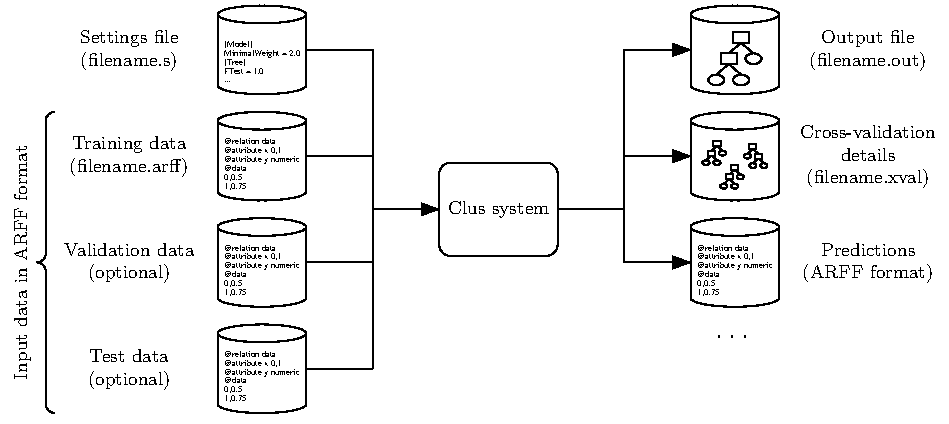
\includegraphics{fig/clusinout}
\caption{\label{fig:iofiles}Input and output files of Clus.}
\end{figure}

\begin{figure}[tb]
\hrule
\begin{verbatim}
[Attributes]
Descriptive = 1-2
Target = 3-4
Clustering = 3-4

[Tree]
Heuristic = VarianceReduction
\end{verbatim}
\hrule
\caption{The settings file (weather.s) for the Weather example.}
\label{weathers:fig}
\end{figure}
\begin{figure}[tb]
\hrule
\begin{verbatim}
@RELATION "weather"

@ATTRIBUTE outlook     {sunny,rainy,overcast}
@ATTRIBUTE windy       {yes,no}
@ATTRIBUTE temperature numeric
@ATTRIBUTE humidity    numeric

@DATA
sunny,    no,  34, 50
sunny,    no,  30, 55
overcast, no,  20, 70 
overcast, yes, 11, 75
rainy,    no,  20, 88
rainy,    no,  18, 95 
rainy,    yes, 10, 95 
rainy,    yes, 8,  90
\end{verbatim}
\hrule
\caption{The training data (weather.arff) for the Weather example (in Weka's ARFF format).}
\label{weatherarff:fig}
\end{figure}

\begin{figure}[tb]
\hrule
\begin{verbatim}
Clus run "weather"
******************
Date: 1/10/10 12:23 PM
File: weather.out
Attributes: 4 (input: 2, output: 2)

[Data]
File = weather.arff

[Attributes]
Target = 3-4
Clustering = 3-4
Descriptive = 1-2

[Tree]
Heuristic = VarianceReduction
PruningMethod = M5

Statistics
----------
Induction Time: 0.017 sec
Pruning Time: 0.001 sec
Model information
     Original: Nodes = 7 (Leaves: 4)
     Pruned: Nodes = 3 (Leaves: 2)

Training error
--------------
Number of examples: 8
Mean absolute error (MAE)
   Default        : [7.125,14.75]: 10.9375
   Original       : [2.125,2.75]: 2.4375
   Pruned         : [4.125,7.125]: 5.625
Mean squared error (MSE)
   Default        : [76.8594,275.4375]: 176.1484
   Original       : [6.5625,7.75]: 7.1562
   Pruned         : [19.4375,71.25]: 45.3438

Original Model
**************
outlook = sunny
+--yes: [32,52.5]: 2
+--no:  outlook = rainy
        +--yes: windy = yes
        |       +--yes: [9,92.5]: 2
        |       +--no:  [19,91.5]: 2
        +--no:  [15.5,72.5]: 2

Pruned Model
************
outlook = sunny
+--yes: [32,52.5]: 2
+--no:  [14.5,85.5]: 6
\end{verbatim}
\hrule
\caption{The Weather example's output (weather.out). (Some parts have been omitted for brevity.)}
\label{weatherout:fig}
\end{figure}

\clus{} uses (at least) two input files and these are named {\tt {\em filename}.s} and {\tt {\em filename}.arff}, with {\tt {\em filename}} a name chosen by the user.  The file {\tt {\em filename}.s} contains the parameter settings for \clus{}.  The file {\tt {\em filename}.arff} contains the training data to be read. The format of the data file is Weka's ARFF format\footnote{\url{http://weka.wikispaces.com/ARFF}}. The results of a \clus{} run are put in an output file {\tt {\em filename}.out}. Figure~\ref{fig:iofiles} gives an overview of the input and output files supported by \clus{}. The format of the data files is described in detail in Chapter~\ref{ch:data}, the format of the settings file is discussed in Chapter~\ref{ch:sett}, and the output files are covered in Chapter~\ref{ch:output}. 

In the Weather example of Section~\ref{sec:run}, \clus{} will read its settings from the input file ``weather.s'' (shown in Figure~\ref{weathers:fig}) and its input data from the file ``weather.arff'' (Figure~\ref{weatherarff:fig}). It will then construct (with these settings) a PCT, which it will write to the output file ``weather.out'' (Figure~\ref{weatherout:fig}).

The Weather example is a small multi-target or multi-task learning problem \cite{Caruana97:jrnl} in which the goal is to predict the target attributes temperature and humidity from the input attributes outlook and windy. The details about the learning task are specified in the settings file (Figure~\ref{weathers:fig}). Our example includes values for four parameters. The parameters under the heading ``[Attributes]'' specify how the attributes are to be used. Here, the first two attributes (attributes 1-2) are to be used in the cluster descriptions, that is, in the tests that appear in the PCT's nodes. The last two attributes (attributes 3-4) are to be predicted. The setting ``Clustering = 3-4'' indicates that the clustering heuristic, which is used to construct the PCT, should be computed based on the target attributes only. Finally, ``Heuristic = VarianceReduction'' specifies that the heuristic is variance reduction. Chapter~\ref{ch:sett} provides a detailed description of each setting supported by \clus{}.

\clus{} writes the resulting PCT together with a number of statistics such as the training set error and the test set error (if a test set has been provided) to its output file (Figure~\ref{weatherout:fig}).  In this example, the resulting tree is a multi-target tree: each leaf predicts a vector of which the first component is the predicted temperature and the second component the predicted humidity. Such a multi-target tree has several advantages over constructing a separate regression tree for each target variable. The most obvious one is the number of models: the user only has to interpret one tree instead of at one tree for each target. A second advantage is that the tree makes features that are relevant to all target variables explicit. For example, the first leaf of the tree in Figure~\ref{weatherout:fig} shows that ``outlook = sunny'' implies both a high temperature and a low humidity. Finally, due to the concept of inductive transfer, multi-target PCTs may also be more accurate than regression trees. More information about multi-target trees can be found in the following publications: \cite{Blockeel1998icml, Blockeel99:proc, Struyf06-KDID:proc, Piccart08-DS-:proc}.

% \chapter{Learning Algorithms}
% 
% \section{Tree Learning}
% 
% \subsection{Top-down Induction}
% 
% \subsection{Beam Search}
% 
% \subsection{Constrained Induction}
% 
% \subsection{Ensembles}
% 
% \section{Rule Learning}
% 
% \subsection{Sequential Covering Algorithm}
% 
% \subsection{Rule Ensembles}
% 
% \chapter{Case Studies}
%  
% \section{Multi-target Regression and Classification}
% 
% \section{Hierarchical Multi-label Classification}
% 
% \section{Time Series Clustering}
% 
% \section{Clustering with Instance Level Constraints}

\chapter{Input Format}
\label{ch:data}

Like many machine earning systems, Clus learns from tabular data.
These data are assumed to be in the ARFF format that is also used by the Weka data mining tool.  Full details on ARFF can be found elsewhere\footnote{\url{http://weka.wikispaces.com/ARFF}}.
We here only give a minimal description.

In the data table, each row represents an instance, and each column represents an attribute of the instances.  Each attribute has a name and a domain (the domain is the set of values it can take).  In the ARFF format, the names and domains of the attributes are declared up front, before the data are given.

An ARFF file follows the following format:

\begin{tabbing}
{\tt \% all comment lines are optional, start with \%, and can occur }\\
{\tt \% anywhere in the file}\\
\\
{\tt @RELATION} name\\
\\
{\tt @ATTRIBUTE} name domain\\
{\tt @ATTRIBUTE} name domain\\
...\\
\\
{\tt @DATA}\\
value$_1$, value$_2$, ..., value$_n$\\
value$_1$, value$_2$, ..., value$_n$\\
\end{tabbing}

The domain of an attribute can be one of:
\begin{tabbing}
\tt real\\
{\tt \{ } nomvalue$_1$, nomvalue$_2$, ..., nomvalue$_n$ {\tt \} }\\
{\tt hierarchical} hvalue$_1$, hvalue$_2$, ..., hvalue$_n$
\end{tabbing}

The first option, {\tt real}, indicates that the domain is the set of real numbers.

The second type of domain is called a discrete domain.  Discrete domains are defined by enumerating the values they contain.  These values are nominal.

The third type of domain is called ``hierarchical multi-label".  It implies two things: first, the attribute takes as value a {\em set} of values from the domain, rather than a single value; second, the domain has a hierarchical structure.  The elements of the domain are typically denoted $v_1/v_2/.../v_i$ with $i \leq d$ where $d$ is the depth of the hierarchy.  This type of domain is useful in the context of hierarchical multi-label classification.  

The values in a	 row occur in the same order as the attributes: the $i$'th value is assigned to the $i$'th attribute.  Values in the rows must be real values if the domain of the corresponding attribute is continuous, or a member of the specified set of values if the domain is discrete.  For hierarchical multi-label attributes, a set of values from the domain can be given; this set is written by listing its elements separated by \verb^@^.

Figure~\ref{weatherarff:fig} shows an example of an ARFF file. An example of a table containing hierarchical multi-label attributes is shown in Figure~\ref{arffhmc:fig}. Finally, an ARFF file with a time series attribute is shown in Figure~\ref{arfftimeser:fig}.

\begin{figure}[tb]
\hrule
\begin{verbatim}
@RELATION HMCNewsGroups

@ATTRIBUTE word1   {1,0}
...
@ATTRIBUTE word100 {1,0}
@ATTRIBUTE class hierarchical rec/sport/swim,rec/sport/run,rec/auto,alt/atheism,...

@DATA
1,...,1,rec/sport/swim
1,...,1,rec/sport/run
1,...,1,rec/sport/run@rec/sport/swim
1,...,0,rec/sport
1,...,0,rec/auto
0,...,0,alt/atheism
...
\end{verbatim}
\hrule
\caption{An ARFF file that includes an hierarchical multi-label attribute.}
\label{arffhmc:fig}
\end{figure}

\begin{figure}[tb]
\hrule
\begin{verbatim}
@RELATION GeneExpressionTimeSeries

@ATTRIBUTE geneid string
@ATTRIBUTE GO0000003 {1,0}
@ATTRIBUTE GO0000004 {1,0}
...
@ATTRIBUTE GO0051704 {1,0}
@ATTRIBUTE GO0051726 {1,0}
@ATTRIBUTE target timeseries

@DATA
YAL001C,0,0,0,0,0,0,0,0,0,0,0,0,0,...,0,0,0,0,[0.07, 0.15, 0.14, 0.15,-0.11, 0.07,-0.41]
YAL002W,0,0,0,0,0,0,0,0,0,0,1,0,0,...,1,1,0,0,[0.14, 0.14, 0.18, 0.14, 0.17, 0.13, 0.07]
YAL003W,0,0,0,0,0,0,0,0,0,0,0,0,0,...,0,0,0,0,[0.46, 0.33, 0.04,-0.60,-0.64,-0.51,-0.36]
YAL005C,0,0,0,0,0,0,0,0,0,0,0,0,0,...,1,1,0,0,[0.86, 1.19, 1.58, 0.93, 1,    0.85, 1.24]
YAL007C,0,0,0,0,0,0,0,0,0,0,0,0,0,...,1,1,0,0,[0.12, 0.49, 0.62, 0.49, 0.84, 0.89, 1.08]
YAL008W,0,1,0,0,0,0,0,0,0,0,0,0,0,...,0,0,0,0,[0.49, 1.01, 1.33, 1.23, 1.32, 1.03, 1.14]
...
\end{verbatim}
\hrule
\caption{An ARFF file that includes an time series attribute.}
\label{arfftimeser:fig}
\end{figure}

\begin{figure}[tb]
\hrule
\begin{verbatim}
@RELATION SparseData

@ATTRIBUTE a1    numeric
@ATTRIBUTE a2    numeric
...
@ATTRIBUTE a10   numeric
@ATTRIBUTE a11   numeric
@ATTRIBUTE class {pos,neg}

@DATA
{1 3.1, 8 2.5, 12 pos}
{7 2.3, 12 neg}
{2 8.5, 3 1.3, 12 neg}
{1 3.2, 12 pos}
{1 3.3, 8 2.7, 12 pos}
...
\end{verbatim}
\hrule
\caption{An ARFF file in sparse format.}
\label{arffsparse:fig}
\end{figure}

\chapter{Settings File}
\label{ch:sett}

The algorithms included in the \clus{} system have a number of parameters that influence their behavior.  Most parameters have a default setting; the specification of a value for such parameters is optional.  For parameters that do not have a default setting or which should get another value than the default, a value must be specified in the settings file, {\tt {\em filename}.s}.

The settings file is structured into sections.  Each parameter belongs to a particular section.  Including the section headers is optional, however; these sections are meant to help users structure the settings file but are not mandatory.

We here explain the most common settings.  Figure~\ref{settings:fig} shows how they might occur in a settings file.

In the following, we use the convention that $n$ is an integer, $r$ is a real, $v$ is a vector of real values, $s$ is a string, $y$ is an element of \{ {\tt Yes}, {\tt No} \}, $r$ is an range of attribute indices, and $o$ is another type of value.  Strings are denoted without quotes. A vector is denoted as $[r_1,\ldots,r_n]$. An attribute range is a comma separated list of integers or intervals or \texttt{None} if the range is empty. For example, {\tt 5,7-9} indicates attributes 5, 7, 8 and 9. The first attribute in the dataset is attribute 1. Run {\tt clus -info {\em filename}.s} to list all attributes together with their indices.

\section{General}

\begin{itemize}
\item {\tt RandomSeed = $n$}\label{sett:seed} : $n$ is used to initialize the random generator.
Some procedures used by \clus{} (e.g., creation of cross-validation folds) are randomized, and as a result, different runs of \clus{} on identical data may still yield different outputs.  When \clus{} is run on identical input data with the same {\tt RandomSeed} setting, it is guaranteed to yield the same results.
\end{itemize}

\section{Data}

\begin{itemize}
\item {\tt File = $s$} : $s$ is the name of the file that contains the training set.  The default value for $s$ is {\tt {\em filename}.arff}.  \clus{} can read compressed ({\tt .arff.zip}) or uncompressed ({\tt .arff}) data files.
\item {\tt TestSet = $o$} : when $o$ is {\tt None}, no test set is used; if $o$ is a number between 0 and 1, \clus{} will use a proportion $o$ of the data file as a separate test set (used for evaluating the model but not for training); if $o$ is a valid file name containing a test set in ARFF format, \clus{} will evaluate the learned model on this test set.
\item {\tt PruneSet = $o$} : defines whether and how to use a pruning set; the meaning of $o$ is identical as in the {\tt TestSet} setting
\item {\tt XVal = $n$}\label{sett:xval} : $n$ is the number of folds to be used in a cross-validation.  To perform cross-validation, \clus{} needs to be run with the {\tt -xval} option.
\end{itemize}

\section{Attributes}

\begin{itemize}
\item {\tt Target = $r$} : sets the range of target attributes. The predictive clustering model will predict these attributes. If this setting is not specified, then it is equal to the index of the last attribute in the training dataset, i.e., the last attribute is the target by default. This setting overrides the \texttt{Disable} setting. This is convenient if one needs to build models that predict only a subset $S$ of all available target attributes $T$. Because {\tt Target} overrides {\tt Disable}, one can use the settings {\tt Disable = $T$} and {\tt Target = $S$} to this end. 

\item {\tt Clustering = $r$} : sets the range of clustering attributes. The predictive clustering heuristic that is used to guide the model construction is computed with regard to these atrributes. If this setting is not specified, then the clustering attributes are by default equal to the target attributes.

\item {\tt Descriptive = $r$} : sets the range of attributes that can be used in the descriptive part of the models. For a PCT, these attributes will be used to construct the tests in the internal nodes of the tree. For a set of PCRs, these attributes will appear in the rule conditions. If this setting is not specified, then the descriptive attributes are all attributes that are not target, key, or disabled.

\item {\tt Disable = $r$} : sets the range of attributes that are to be ignored by Clus. These attributes are also not read into memory.

\item {\tt Key = $r$} : sets the range of key attributes. A key attribute or a set of key attributes can be used as an example identifier. For example, if each instance represents a person, then the key attribute could store the person's name. Key attributes are not actually used by the induction algorithm, but they are written to output files, for example, to ARFF files with predictions. See \texttt{[Output]/WritePredictions} for an example.

\item {\tt Weights = $o$} : sets the relative weights of the different attributes in the clustering heuristic. To set the weights of all clustering attributes to 1.0, use {\tt Weights = 1}. To use as  weights $w_i = 1/\mathrm{Var}(a_i)$, with $\mathrm{Var}(a_i)$ the variance of attribute $a_i$ in the input data, use {\tt Weights = Normalize}.
\end{itemize}

\section{Model}

\begin{itemize}
\item {\tt MinimalWeight = $r$} : \clus{} only generates splits with at least $r$ instances in each subset.
\end{itemize}

\section{Tree}

\begin{itemize}
\item {\tt FTest = $r$} : sets the f-test stopping criterion for regression; a node will only be split if a statistical F-test indicates a significant (at level $r$) reduction of variance inside the subsets.
\item {\tt ConvertToRules = $y$} : If {\tt Yes},  \clus{} will convert the induced tree to a set of rules.
\end{itemize}

\section{Rules}


\section{Ensembles}

\section{Constraints}

\begin{itemize}
\item {\tt Syntactic = $o$} : sets the file with syntactic constraints (e.g., a partial tree) \cite{Struyf06-KDID:proc}
\item {\tt MaxSize = $o$} : sets the maximum size for Garofalakis pruning \cite{Garofalakis03:jrnl, Struyf06-KDID:proc}; $o$ can be a positive integer or {\tt Infinity}
\item {\tt MaxError = $o$} : sets the maximum error for Garofalakis pruning; $o$ is a positive real or {\tt Infinity}
\item {\tt MaxDepth = $o$} : $o$ is a positive integer or {\tt Infinity}. \clus{} will build trees with depth at most $o$.
\end{itemize}

\section{Output}

\begin{itemize}
\item {\tt AllFoldModels = $y$} : if set to {\tt Yes}, \clus{} will output the model built in each fold of a cross-validation
\item {\tt AllFoldErrors = $y$} : if set to {\tt Yes}, \clus{} will output the test set error (and other evaluation measures) for each fold
\item {\tt TrainErrors = $y$} : if set to {\tt Yes}, \clus{} will output the training set error (and other evaluation measures)
\item {\tt UnknownFrequency = $y$} : if set to {\tt Yes}, \clus{} will show in each node of the tree the proportion of instances that had a missing value for the test in that node
\item {\tt BranchFrequency = $y$} : if set to {\tt Yes}, \clus{} will show in each node of the tree, for each possible outcome of the test in that node, the proportion of instances that had that outcome
\item {\tt WritePredictions = $o$} : $o$ is a subset of \{Train,Test\}. If $o$ includes ``Train'', then the prediction for each training instance will be written to an ARFF output file. The file is named {\tt {\em filename}.train.{\em i}.pred.arff} with $i$ the iteration. In a single run, $i = 1$. In a 10 fold cross-validation, $i$ will vary from 1 to 10. If $o$ includes ``Test'', then the predictions for each test instance will be written to disk. The file is named {\tt {\em filename}.test.pred.arff}.
\end{itemize}

\section{Beam}

\begin{itemize}
\item {\tt SizePenalty = $o$} : sets the size penalty parameter used in the beam heuristic \cite{Kocev07a:proc}
\item {\tt BeamWidth = $n$} : sets the width of the beam used in the beam search performed by \clus{} \cite{Kocev07a:proc}
\item {\tt MaxSize = $o$} : sets the maximum size constraint \cite{Kocev07a:proc}; $o$ is a positive integer or {\tt Infinity}
\end{itemize}

\begin{figure}[tb]
\hrule
\begin{verbatim}
[General]
RandomSeed = 0              % seed of random generator

[Data]
File = weather.arff         % training data
TestSet = None              % data used for evaluation (file name / proportion)
PruneSet = None             % data used for tree pruning (file name / proportion)
XVal = 10                   % number of folds in cross-validation (clus -xval ...)

[Attributes]
Target = 5                  % index of target attributes
Disable = 4                 % Disables some attributes (e.g., "5,7-8")
Key = None                  % Sets the index of the key attribute
Weights = Normalize         % Normalize numeric attributes

[Model]
MinimalWeight = 2.0         % at least 2 examples in each subtree
         
[Tree]
FTest = 1.0                 % f-test stopping criterion for regression
ConvertToRules = No         % Convert the tree to a set of rules

[Constraints]
Syntactic = None            % file with syntactic constraints (a partial tree)
MaxSize = Infinity          % maximum size for Garofalakis pruning
MaxError = Infinity         % maximum error for Garofalakis pruning
MaxDepth = Infinity         % Stop building the tree at the given depth

[Output]
AllFoldModels = Yes         % Output model in each cross-validation fold
AllFoldErrors = No          % Output error measures for each fold
TrainErrors = Yes           % Output training error measures
UnknownFrequency = No       % proportion of missing values for each test
BranchFrequency = No        % proportion of instances for which test succeeds
WritePredictions = {Train,Test}    % write test set predictions to file

[Beam]
SizePenalty = 0.1           % size penalty parameter used in the beam heuristic
BeamWidth = 10              % beam width
MaxSize = Infinity          % Sets the maximum size constraint
\end{verbatim}
\hrule
\caption{An example settings file}
\label{settings:fig}
\end{figure}


\section{Hierarchical}

A number of settings are relevant only when using \clus{} for Hierarchical Multi-label Classification (HMC).  These go in the separate section ``Hierarchical''.  The most important ones are:

\begin{itemize}
\item {\tt Type = $o$} : $o$ is {\tt Tree} or {\tt DAG}, and indicates whether the class hierarchy is a tree or a directed acyclic graph \cite{Vens08:jrnl}
\item {\tt WType = $o$} : defines how parents' class weights are aggregated in DAG-shaped hierarchies (\cite{Vens08:jrnl}, Section 4.1): possible values are {\tt ExpSumParentWeight}, {\tt ExpAvgParentWeight}, {\tt ExpMinParentWeight}, {\tt ExpMaxParentWeight}, and {\tt NoWeight}.  These define the weight of a class to be $w_0$ times the sum, average, minimum or maximum of the parent's weights, respectively, or to be 1.0 for all classes. 
\item {\tt WParam = $r$} : sets the parameter $w_0$ used in the formula for defining the class weights (\cite{Vens08:jrnl}, Section 4.1)
\item {\tt HSeparator = $o$} : $o$ is the separator used in the notation of values of the hierarchical domain (typically `/' or `.') 
\item {\tt EmptySetIndicator = $o$} : $o$ is the symbol used to indicate the empty set
\item {\tt OptimizeErrorMeasure = $o$} : \clus{} can automatically optimize the {\tt FTest} setting; $o$ indicates what criterion should be maximized for this (\cite{Vens08:jrnl}, Section 5.2).  Possible values for $o$ are:
  \begin{itemize}
   \item {\tt AverageAUROC}: average of the areas under the class-wise ROC curves
   \item {\tt AverageAUPRC}: average of the areas under the class-wise precision-recall curves
   \item {\tt WeightedAverageAUPRC}: similar to AverageAUPRC, but each class's contribution is weighted by its relative frequency
   \item {\tt PooledAUPRC}: area under the average (or pooled) precision-recall curve
  \end{itemize}
\item {\tt ClassificationThreshold = $o$} : The original tree constructed by \clus{} contains a vector of predicted probabilities (one for each class) in each leaf. Such a probabilistic prediction can be converted into a set of labels by applying a threshold $t$: all labels that are predicted with probability $\geq t$ are in the predicted set.  $o$ can be a list of thresholds, e.g., [0.5, 0.75, 0.80, 0.90, 0.95]. \clus{} will output for each value in the set a tree in which the predicted label sets are constructed with this particular threshold. So, in the example, the output file will contain 5 trees corresponding to the thresholds 0.5, 0.75, 0.80, 0.90 and 0.95.

\item {\tt RecallValues = $o$} : $o$ is a list of recall values, e.g., [0.1, 0.2, 0.3]. For each value, \clus{} will output the average of the precisions over all class-wise precision-recall curves that correspond to the particular recall value in the output file.
\item {\tt EvalClasses = $o$} : If $o$ is {\tt None}, \clus{} computes average error measures across all classes in the class  hierarchy. If $o$ is a list of classes, then the error measures are only computed with regard to the classes in this list.
\end{itemize}

Figure~\ref{settings-hmc:fig} summarizes these briefly.

\begin{figure}[tb]
\hrule
\begin{verbatim}
[Hierarchical]
Type = Tree                         % Tree or DAG hierarchy?
WType = ExpAvgParentWeight          % aggregation of class weights
WParam = 0.75                       % parameter w_0
HSeparator = /                      % separator used in class names
EmptySetIndicator = n               % symbol for empty set
OptimizeErrorMeasure = PooledAUPRC  % FTest optimization strategy
ClassificationThreshold = None      % threshold for "positive"
RecallValues = None                 % where to report precision
EvalClasses = None                  % classes to evaluate
\end{verbatim}
\hrule
\caption{Settings specific for hierarchical multi-label classification}
\label{settings-hmc:fig}
\end{figure}

\chapter{Command Line Parameters}
\label{param:ch}

\clus{} is run from the command line.  It takes a number of command line parameters that affect its behavior.

\begin{itemize}
\item {\tt -xval} : in addition to learning a single model from the whole input dataset, perform a cross-validation.  The XVal setting (page~\pageref{sett:xval}) determines the number of folds; the RandomSeed setting (page~\pageref{sett:seed}) initializes the random generator that determines the folds.

\item {\tt -fold} $N$: run only fold $N$ of the cross-validation.

\item {\tt -rules} : construct predictive clustering rules (PCRs) instead of predictive clustering trees (PCTs).

\item {\tt -forest} : construct an ensemble instead of a single tree \cite{Kocev07b:proc}.

\item {\tt -beam} : construct a tree using beam search \cite{Kocev07a:proc}.

\item {\tt -sit} : run Empirical Asymmetric Selective Transfer \cite{Piccart08-DS-:proc}.

\item {\tt -silent} : run \clus{} with reduced screen output.

\item {\tt -info} : gives information and summary statistics about the dataset.
\end{itemize}

%	public final static String[] OPTION_ARGS = { "exhaustive", "xval", "oxval",
%			"target", "disable", "silent", "lwise", "c45", "info", "sample",
%			"debug", "tuneftest", "load", "soxval", "bag", "obag", "show",
%			"knn", "knnTree", "beam", "gui", "fillin", "rules", "weka",
%			"corrmatrix", "tunesize", "out2model", "test", "normalize",
%			"tseries", "writetargets", "fold", "forest", "copying", "sit", "tc" };

\chapter{Output Files}
\label{ch:output}

When \clus{} is finished, it writes the results of the run into an output file with the name
{\tt {\em filename}.out}.  An example of such an output file is shown in Figures \ref{output1:fig} to \ref{output4:fig}.

\begin{figure}[tb]
\hrule
\begin{verbatim}
Clus run "weather"
******************

Date: 1/10/10 4:37 PM
File: weather.out
Attributes: 4 (input: 2, output: 2)
Missing values: No

[General]
Verbose = 1
Compatibility = Latest
RandomSeed = 0
ResourceInfoLoaded = No

[Data]
File = weather.arff
TestSet = None
PruneSet = None
XVal = 10
RemoveMissingTarget = No
NormalizeData = None

[Attributes]
Target = 3-4
Clustering = 3-4
Descriptive = 1-2
Key = None
Disable = None
Weights = Normalize
ClusteringWeights = 1.0
ReduceMemoryNominalAttrs = No

[Constraints]
Syntactic = None
MaxSize = Infinity
MaxError = 0.0
MaxDepth = Infinity

[Output]
ShowModels = {Default, Pruned, Others}
TrainErrors = Yes
ValidErrors = Yes
TestErrors = Yes
AllFoldModels = Yes
AllFoldErrors = No
AllFoldDatasets = No
UnknownFrequency = No
BranchFrequency = No
ShowInfo = {Count}
PrintModelAndExamples = No
WriteErrorFile = No
WritePredictions = {None}
WriteModelIDFiles = No
WriteCurves = No
OutputPythonModel = No
OutputDatabaseQueries = No
\end{verbatim}
\hrule
\caption{Example output file (part 1, settings).}
\label{output1:fig}
\end{figure}

\begin{figure}[tb]
\hrule
\small
\begin{verbatim}
[Nominal]
MEstimate = 1.0

[Model]
MinimalWeight = 2.0
MinimalNumberExamples = 0
MinimalKnownWeight = 0.0
ParamTuneNumberFolds = 10
ClassWeights = 0.0
NominalSubsetTests = Yes

[Tree]
Heuristic = VarianceReduction
PruningMethod = M5
M5PruningMult = 2.0
FTest = 1.0
BinarySplit = Yes
ConvertToRules = No
AlternativeSplits = No
Optimize = {}
MSENominal = No
\end{verbatim}
\hrule
\caption{Example output file (part 2, settings (ctd.)).}
\label{output2:fig}
\end{figure}

\begin{figure}[tb]
\hrule
\footnotesize
\begin{verbatim}
Run: 01
*******

Statistics
----------

FTValue (FTest): 1.0
Induction Time: 0.018 sec
Pruning Time: 0.001 sec
Model information
     Default: Nodes = 1 (Leaves: 1)
     Original: Nodes = 7 (Leaves: 4)
     Pruned: Nodes = 3 (Leaves: 2)

Training error
--------------

Number of examples: 8
Mean absolute error (MAE)
   Default        : [7.125,14.75]: 10.9375
   Original       : [2.125,2.75]: 2.4375
   Pruned         : [4.125,7.125]: 5.625
Mean squared error (MSE)
   Default        : [76.8594,275.4375]: 176.1484
   Original       : [6.5625,7.75]: 7.1562
   Pruned         : [19.4375,71.25]: 45.3438
Root mean squared error (RMSE)
   Default        : [8.7669,16.5963]: 13.2721
   Original       : [2.5617,2.7839]: 2.6751
   Pruned         : [4.4088,8.441]: 6.7338
Weighted root mean squared error (RMSE) (Weights [0.013,0.004])
   Default        : [1,1]: 1
   Original       : [0.2922,0.1677]: 0.2382
   Pruned         : [0.5029,0.5086]: 0.5058
Pearson correlation coefficient
   Default        : [?,?], Avg r^2: ?
   Original       : [0.9564,0.9858], Avg r^2: 0.9432
   Pruned         : [0.8644,0.861], Avg r^2: 0.7442
\end{verbatim}
\hrule
\caption{Example output file (part 3, statistics).}
\label{output3:fig}
\end{figure}

\begin{figure}[tb]
\hrule
\begin{verbatim}
Default Model
*************

[18.875,77.25]: 8

Original Model
**************

outlook = sunny
+--yes: [32,52.5]: 2
+--no:  outlook = rainy
        +--yes: windy = yes
        |       +--yes: [9,92.5]: 2
        |       +--no:  [19,91.5]: 2
        +--no:  [15.5,72.5]: 2

Pruned Model
************

outlook = sunny
+--yes: [32,52.5]: 2
+--no:  [14.5,85.5]: 6
\end{verbatim}
\hrule
\caption{Example output file (part 4, learned models).}
\label{output4:fig}
\end{figure}

\section{Used Settings}

The first part of {\tt {\em filename}.out} (shown in Figures \ref{output1:fig} and \ref{output2:fig}) contains the values of the settings that were used for this run of \clus{}, in the format used by the settings file.  This part can be copied and pasted to {\tt {\em filename}.s} and modified for subsequent runs.

\section{Evaluation Statistics}

The next part contains statistics about the results of this \clus{} run.

Summary statistics about the running time of \clus{} and about the size of the resulting models are given.  Next, information on the models' predictive performance on the training set (``training set error") is given, as well as an estimate of its predictive performance on unseen examples (``test set error"), when available (this is the case if a cross-validation or an evaluation on a separate test set was performed).  

Typically three models are reported: a ``default'' model consisting of a tree of size zero, which can be used as a reference point (for instance, its predictive accuracy equals that obtained by always predicting the majority class); an unpruned (``original") tree, and a pruned tree.

For classification trees the information given for each model by default includes a contingency table, and (computed from that) the accuracy and Cramer's correlation coefficient.

For regression trees, this information includes the mean absolute error (MAE), mean squared error (MSE), root mean squared error (RMSE), weighted RMSE, the Pearson correlation coefficient $r$ and it square.  In the weighted RMSE, the weight of a given attribute $A$ is its normalization weight, which is $\frac{1}{\sqrt{\mathrm{Var}(A)}}$, with $\mathrm{Var}(A)$ equal to $A$'s variance in the input data. 

\section{The Models}

The output file contains the learned models, represented as decision trees.  The level of detail in which the models are shown is influenced by certain settings.

\chapter{Developer Documentation}
\label{ch:devel}

\section{Compiling Clus}

Note: The \clus{} download comes with a pre-compiled version of \clus{} stored in the file Clus.jar. So, if you just want to run \clus{} as it is on a data set, then you do not need to compile \clus{}. You can run it by following the instructions in Section~\ref{sec:run}. On the other hand, if you wish to modify the source code of \clus{}, or if you are using the CVS version, then you will need to compile the source code of \clus{}. This can be done using the commands
below or using the Eclipse IDE as pointed out in the next section.

(Windows)

\begin{small}
\begin{verbatim}
cd C:\Clus\src
javac -d "bin" -cp ".;jars\commons-math-1.0.jar;jars\jgap.jar" clus/Clus.java
\end{verbatim}
\end{small}

(Unix)

\begin{small}
\begin{verbatim}
cd /home/john/Clus
javac -d "bin" -cp ".:jars/commons-math-1.0.jar:jars/jgap.jar" clus/Clus.java
\end{verbatim}
\end{small}

This will compile \clus{} and write the resulting .class files (Java executable 
byte code) to the "bin" subdirectory.

Alternatively, use the "./compile.sh" script provided in the \clus{} main directory.

\section{Compiling Clus with Eclipse}

In Eclipse, create a new project for \clus{} as follows:

\begin{itemize}
\item Choose \verb^File | New | Project^.
\item Select "Java Project" in the dialog box.
\item In the "New Java Project" dialog box:
 \begin{itemize}
 \item Enter "Clus" in the field "Project Name".
 \item Choose "Create project from existing source" and browse to the location where 
      you unzipped Clus. E.g., \verb^/home/john/Clus^ or \verb^C:\Clus^.
 \item Click "Next".
 \item Select the "Source" tab of the build settings dialog box.
     Change "Default output folder" (where the class files are generated) to: "Clus/bin".
 \item Select the "Libraries" tab of the build settings dialog box.
     Click "Add external jars" and add in this way these three jars:\\
        Clus/jars/commons-math-1.0.jar\\
        Clus/jars/jgap.jar\\
        Clus/jars/weka.jar
 \item Click "Finish".
 \end{itemize}
\item Select the "Navigator" view (Choose Window | Show View | Navigator)
 \begin{itemize}
   \item  Right click the "Clus" project in this view.
   \item  Select "Properties" from the context menu.
   \item  Select the "Java Compiler" tab.
   \item  Set the "Java Compliance Level" to 5.0.
 \end{itemize}
\end{itemize}
Now \clus{} should be automatically compiled by Eclipse.
To run \clus{} from Eclipse:
 \begin{itemize}
   \item Set as main class "clus.Clus".
   \item Set as arguments the name of your settings file (appfile.s).
   \item Set as working directory, the directory on the file system where your data set is located.
\end{itemize}

\section{Running Clus after Compiling the Source Code}

These instructions are for running \clus{} after you compiled its source code (using the instructions "Compiling Clus" or "Compiling Clus with Eclipse"). To run the pre-compiled version that is available in the file "Clus.jar", see Section~\ref{sec:run}.

(Windows)
\begin{small}
\begin{verbatim}
cd path\to\appfile.s
java -cp "C:\Clus\bin;C:\Clus\jars\commons-math-1.0.jar;C:\Clus\jars\jgap.jar" 
  clus.Clus appfile.s
\end{verbatim}
\end{small}

(Unix)

\begin{small}
\begin{verbatim}
cd path/to/appfile.s
java -cp "$HOME/Clus/bin:$HOME/Clus/jars/commons-math-1.0.jar:$HOME/Clus/jars/jgap.jar" 
  clus.Clus appfile.s
\end{verbatim}
\end{small}

Alternatively, use the "./clus.sh" script provided in the \clus{} main directory after adjusting the line that defines CLUS\_DIR at the top of the script.

\bibliographystyle{plain}
\bibliography{.mlbib}

\end{document}
